\chapter{Architecture}

\section{Design of the Hashing Accelerator}

Write about the hashing accelerator architecture here.

\subsection{Theoretical Maximum Performance}\todo{Introduce the modules first}

The hashing modules can finish one round of hashing in 65 clock cycles. If
every hash can be obtained from only one block of data, it is possible to
obtain a hash every 65 clock cycles under ideal conditions. This translates
into a maximum theoretical performance of 768230~H/s at a clock frequency of
50~MHz.

However, the modules do not exist in a vacuum, and data needs to be transferred
between the modules and a controller, such as a microprocessor. The hashing tiles
are connected to the rest of the system using an AXI4 lite interface. Transfers
on the AXI bus takes at least three cycles for writes and two cycles for reads.
It is assumed that no burst transfers are used and that only one transaction
can be executed at a time, corresponding with the requirements for the interface.

In order for the hashing module to work, it needs 16 32-bit words of input data,
and control signals must be set up. This causes at least 17 words of data to
need to be written to the module, taking at least 51 clock cycles. Then, after
hashing of a block is complete, if there are no more blocks, the result must
be read back. The result consists of 8 words of data, which takes at least 16
clock cycles to transfer.

In total, a minimum of 67 clock cycles of overhead is needed per hash when assuming
a one-block input size and an ideal AXI4 bus. Not considering the additional overhead
from processing in the microprocessor, such as when handlig the interrupt when the
hashing finishes, hashing may take a minimum of $67 + 65 = 132$ clock cycles to
complete, bringing the maximum theoretical performance down to at most 378787~H/s.


\section{Design of the DMA Module}
\label{sec:dma-architecture}

\subsection{Assumptions}
To simplify the design of the DMA module, some assumptions as to the system where the
DMA is implemented needs to be done.

It is assumed that all data is transferred sequentially. This is especially important when
it comes to future integration into the SHMAC system, because of the XY routing that the
system uses. However, such an assumption also significantly simplifies the design of the
DMA for use in shared-bus systems.

\subsection{Design requirements}

It was decided on a couple of requirements for the DMA implementation.

\begin{description}
	\item[Use block-to-block transfers.] This is a minimum requirement for being
	able to transfer any amount of data from location A to B.
	\item[Two channels.] This allows the DMA to have two separate transfers going
	at the same time.
	\item[Automatic channel allocation.] Channel allocation is done in hardware,
	saving the CPU from the overhead of allocating and managing channels in software.
	% I removed component-based implementation, because _every_ hardware design is component based. -K.
\end{description}

\subsection{DMA Architecture}
The DMA module consists of several main components: a FIFO buffer that contains transfer
requests from the CPU, a main controller that processes the requests, and two channels
where the memory transfers are executed. The two channels work on independent transfer
tasks. An arbiter is used to control access to the bus interface for the two channels.
An overview of the DMA architecture can be seen in figure \ref{fig:DMATopView}.
\todo{CNTR = counter --- CTRL = controller, please fix the figure}

\begin{figure}[htb]
    \centering
    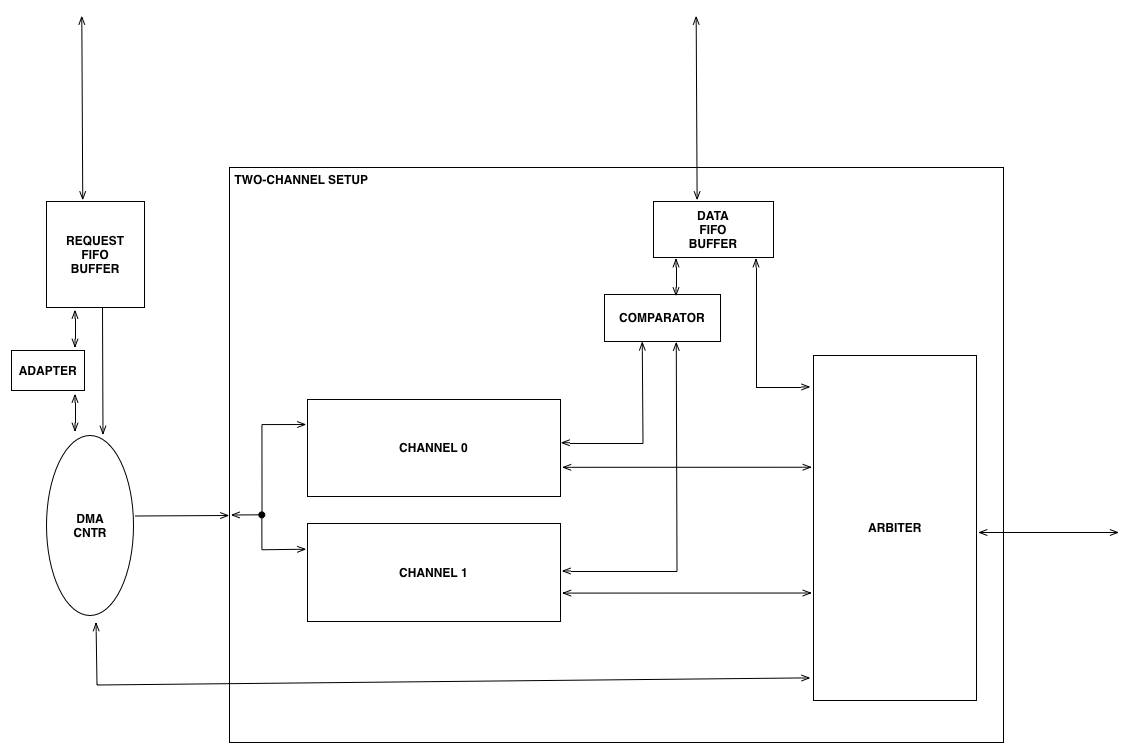
\includegraphics[width=0.8\textwidth]{Figures/DMA/TopViewFinalSimple}
    \caption{DMA module overview}
    \label{fig:DMATopView}
\end{figure}

\subsubsection{Main Controller}
The role of the main controller is to process incoming transfer requests, allocate and activate
channels that are free to execute requests, monitor the channels, and send out an interrupt signal
when a transfer is completed. 

The controller is implemented as a simple state machine, shown in figure \ref{fig:DMAControllerStateMachine}.

\begin{figure}[htb]
    \centering
    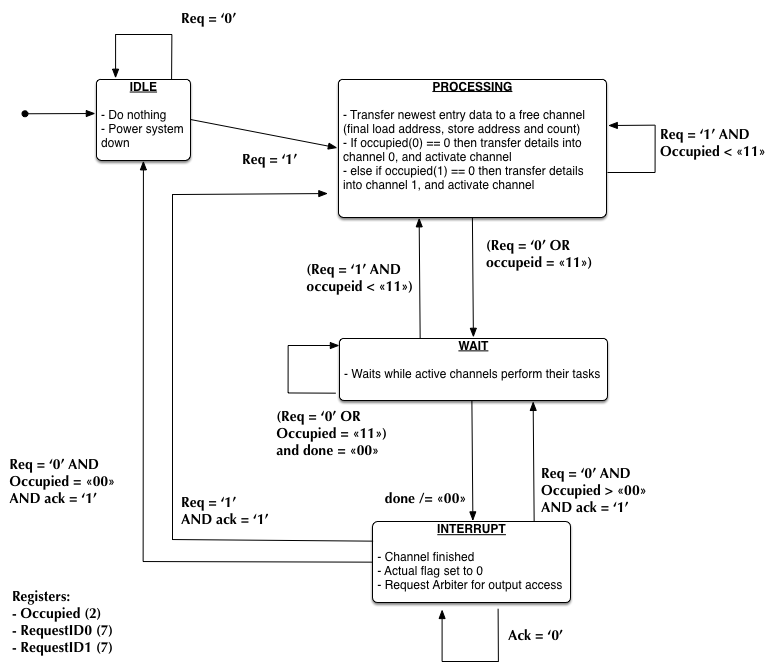
\includegraphics[width=0.8\textwidth]{Figures/DMA/StateMachineFinal}
    \caption{DMA Controller State Machine}
    \label{fig:DMAControllerStateMachine}
\end{figure}

\subsubsection{Channels}
A channel is split into two parts: a part that is responsible for sending out load
commands, and a storing part that issues a store commands. These ``subchannels''
are called the load channel and store channel, respectively.
\todo{Perhaps add an overview picture of channels here}

\subsubsection{Bus interaction system}
In order for the DMA module to be as general as possible, it contains only a general
interface for communicating with a bus system. An adapter is then used to connect
the module to the bus system. This makes it possible to use the DMA module without
changes in either SHMAC or a shared-bus system.

\section{Alternative Simplified Designs} 

In order for the design to be more appropriate for environments where there are
constraints on, for example, logic resources or size of the module, certain simplifications
are possible.

\todo{Consider making diagrams to show the alternatives}

\subsection{Reducing the Controller Logic}
It is possible to remove some of the main components from the DMA module and still
have a functional DMA Module. The request FIFO and the DMA controller could be removed,
and a channel could be directly connected to the bus interface adapter with little
extra work.

This would slightly reduce the number of cycles that is needed to process a request.
The system would also be smaller, including less combinatorics and registers.

On the other hand, this makes the DMA Module much more dependent on the external system, since requests are processed and set externally, not by the DMA Module itself.
Futhermore, removing the controller also constricts the possibility for the DMA Module itself to be able to process different types of requests.
In the minimum case, the only requests that it needs to handle are data transfer requests.
But if the DMA Module is implemented in the SHMAC system, and one wants an as efficient data transfer as possible, one have to consider the option of dynamicly forwarding the request.
An example would be forwarding to the DMA Module that is \todo{Mentioned in chapter 3.5.1., see figure 3.3} closest to both source and destination.

Part of the purpose with the design is to make the DMA Module generic, so that it can implemented in different systems.
In order to make the design as generic as possible, a controller and an incoming request FIFO
in case of multiple requests is therefore essential.

\subsection{Using Channels with a Private Data Buffer}
Instead of using a channel with shared data buffer, where the data output owned by
one of the channels is sent straight through the arbiter, it could be sent to a
private buffer inside the correct channel.
\todo{After I reduced this chapter, an explanation of the shared/private buffers will need to be added somewhere}

\todo{Expand when you wake up from bed. Good night}
Pros: Secure data

Cons: More unnecessary combinatorics + no better throughput

